\chapter{تنوّع الكائنات الحية}\label{ch:g12:diversification-of-life}

لقمح الخبز 42 صبغيًا، في ستة أطقم من سبعة: فهو حصيلة ثلاث حشائش برية
تهاجنت، مرتين، في حقول أوائل المزارعين. وللأصلة ثلاثمئة فقرة وللفأر
ثلاثون، ومع ذلك يبنيان عمودهما الفقري \omterm{def:g10:universal-dna:gene}{بالمورّثات} نفسها. والأشنة على
صخرة كائنان اثنان، فطر وطحلب، عاشا واحدًا من الزمن ما لم يعد معه يوجد
أحدهما وحده. والشمبانزي الصغير يتعلم كسر الجوز بحجر بمشاهدة أمه، في
غابة لم يتعلم قط شمبانزيها البعيد مئة كيلومتر ذلك. \omterm{def:g11:mutations:mutation}{فالطفرة} وخلط الفصل
الماضي ليسا الطريقين الوحيدين اللذين تختلف بهما الكائنات الحية؛
ويستعرض هذا الفصل سائر الطرق.

\section{أكثر من الطفرة}

\begin{proposition}[مصادر التنوّع]\label{prop:g12:diversification-of-life:sources}
\omterm{def:g11:mutations:mutation}{الطفرات} النقطية والخلط الجنسي ينشئان \omterm{def:g10:universal-dna:gene}{أليلات} جديدة وتوافيق جديدة منها.
وفيما وراء ذلك، أنتج تنوّع الكائنات الحية بمسارات تغير المجين على
مقياس أكبر --- بمضاعفة \omterm{def:g10:universal-dna:gene}{المورّثات}، وباستيراد \omterm{def:g10:universal-dna:gene}{المورّثات} من \omterm{def:g10:biodiversity-scales:species}{أنواع} أخرى،
وبإضافة أطقم صبغية كاملة --- وبتغيرات في طريقة استعمال \omterm{def:g10:universal-dna:gene}{المورّثات}
الموجودة أثناء النماء، وبارتباطات بين \omterm{def:g10:biodiversity-scales:species}{الأنواع}، وفي الحيوان بسلوك ينتقل
بلا \omterm{def:g10:universal-dna:gene}{مورّثات} البتة.
\end{proposition}
\admitted

\section{مورّثات جديدة من قديمة}

\begin{proposition}[تضاعف المورّثات وتباعدها]\label{prop:g12:diversification-of-life:duplication}
قد يترك تصالب غير متساوٍ (\cref{ch:g12:meiosis-genetic-shuffling}) أو
خطأ في النسخ صبغيًا بنسختين من \omterm{def:g10:universal-dna:gene}{مورّثة}. فتتابع إحدى النسختين عملها
الأصلي؛ وتتراكم في الأخرى، وقد تحررت من ذلك القيد، \omterm{def:g11:mutations:mutation}{طفرات} فتكتسب وظيفة
جديدة --- أو تضيع. وهذا، إذ يتكرر على مدى التطور، ينتج \emph{عائلات
مورّثية}\index{عائلة مورّثية}: أطقمًا من \omterm{def:g10:universal-dna:gene}{مورّثات} متقاربة منحدرة من سلف
واحد، تسجل درجات تشابهها ترتيب التضاعفات.
\end{proposition}
\begin{proof}[شواهد]
الأوبسينات الثلاثة والرودوبسين في \cref{ch:g11:the-eye} عائلة كهذه؛
والغلوبينات عائلة أخرى: \omterm{def:g10:universal-dna:gene}{فمورّثات} سلاسل الخضاب الدموي العدة --- واحدة
تستعمل في الجنين المبكر، وواحدة في الجنين، واثنتان في البالغ ---
\omterm{def:g10:universal-dna:gene}{ومورّثة} الميوغلوبين، وهو مخزن الأكسجين في العضلة، تقع في عناقيد على
صبغيين، وتتطابق تسلسلاتها بنسبة 40\% إلى 80\%، وتوافق شجرتها الترتيب
الذي ظهرت به مجموعات \omterm{def:g10:common-ancestry:bodyplan}{الفقاريات}. وتحمل المجينات مئات العائلات كهذه،
ويتألف جزء معتبر من كل مجين من قطع مضاعفة.
\end{proof}

\begin{omfigure}
\begin{tikzpicture}[font=\small, line cap=round, >=Stealth]
  \tikzset{g/.style={draw, fill=omDef!30, minimum height=0.45cm, minimum width=1.2cm, inner sep=1pt, font=\scriptsize}}
  % step 1: one gene
  \draw[thick] (0,3) -- (4,3); \node[g] at (2,3) {غلوبين};
  \node[anchor=east] at (-0.2,3) {مورّثة سلفية};
  \draw[->, thick] (2,2.65) -- (2,2.15) node[midway, right] {تضاعف};
  % step 2: two identical copies
  \draw[thick] (0,1.8) -- (5.4,1.8); \node[g] at (1.6,1.8) {غلوبين}; \node[g] at (3.4,1.8) {غلوبين};
  \node[anchor=east] at (-0.2,1.8) {نسختان};
  \draw[->, thick] (2.5,1.45) -- (2.5,0.95) node[midway, right] {تتراكم الطفرات في كل منهما};
  % step 3: diverged
  \draw[thick] (0,0.6) -- (5.4,0.6); \node[g, fill=omThm!30] at (1.6,0.6) {غلوبين $\alpha$}; \node[g, fill=omMeth!30] at (3.4,0.6) {غلوبين $\beta$};
  \node[anchor=east] at (-0.2,0.6) {مورّثتان};
  \draw[->, thick] (2.5,0.25) -- (2.5,-0.25) node[midway, right] {تضاعفات أخرى};
  \draw[thick] (0,-0.6) -- (7.6,-0.6);
  \node[g, fill=omThm!30] at (1.0,-0.6) {$\zeta$}; \node[g, fill=omThm!30] at (2.4,-0.6) {$\alpha$};
  \node[g, fill=omMeth!30] at (4.2,-0.6) {$\varepsilon$}; \node[g, fill=omMeth!30] at (5.5,-0.6) {$\gamma$}; \node[g, fill=omMeth!30] at (6.8,-0.6) {$\beta$};
  \node[anchor=east] at (-0.2,-0.6) {عائلة مورّثية};
  \node[anchor=west, align=left, font=\scriptsize] at (7.9,-0.6) {سلاسل الجنين المبكر\\ والجنين والبالغ};
\end{tikzpicture}

{\small كيف تنمو \omterm{prop:g12:diversification-of-life:duplication}{عائلة مورّثية}. تضاعف \omterm{def:g10:universal-dna:gene}{مورّثة} واحدة؛ ثم تتباعد النسختان
\omterm{def:g11:mutations:mutation}{بالطفرات} حتى تؤدي كل منهما عملًا مختلفًا؛ ثم تكرر تضاعفات أخرى المسار.
وتمد عائلة الغلوبين سلاسل مختلفة من الخضاب الدموي في أطوار مختلفة من
الحياة.}
\end{omfigure}

\begin{proposition}[النقل الأفقي للمورّثات]\label{prop:g12:diversification-of-life:horizontal}
تستطيع \omterm{def:g10:universal-dna:gene}{المورّثات} أيضًا أن تدخل مجينًا من \omterm{def:g10:biodiversity-scales:species}{نوع} آخر. فالجراثيم تتبادل
البلازميدات بحرية (\cref{ch:g11:antibiotic-resistance})؛ والفيروسات
تحمل قطعًا من \omterm{def:g10:universal-dna:information}{DNA} مضيفاتها من \omterm{def:g10:cells-common-unit:cell}{خلية} إلى أخرى وتترك وراءها نسخًا من
مورّثاتها؛ وتبين مقارنة المجينات أن الحيوان والنبات كذلك اكتسبا
\omterm{def:g10:universal-dna:gene}{مورّثات} بهذا السبيل. فنحو 8\% من المجين البشري من أصل فيروسي، وواحدة
على الأقل من تلك \omterm{def:g10:universal-dna:gene}{المورّثات}، وقد كانت أداة فيروس لدمج \omterm{def:g10:cells-common-unit:cell}{الخلايا}، تبني
المشيمة اليوم.
\end{proposition}
\admitted

\begin{proposition}[التهجين وتعدد الصيغ الصبغية]\label{prop:g12:diversification-of-life:polyploidy}
قد يتهاجن نوعان متقاربان أحيانًا؛ فيحمل الهجين طقمًا صبغيًا من كل منهما
ويكون عقيمًا عادة، إذ لا شركاء لصبغياته تتزاوج معها في \omterm{def:g12:meiosis-genetic-shuffling:meiosis}{الانقسام
المنصّف}. فإن ضاعف الهجين صبغياته، بخطأ في الانقسام، ظفر كل \omterm{def:g10:universal-dna:information}{صبغي} بشريك،
وعمل \omterm{def:g12:meiosis-genetic-shuffling:meiosis}{الانقسام المنصّف}، ووجد في الحال \omterm{def:g10:biodiversity-scales:species}{نوع} جديد خصيب --- هو \emph{متعدد
الصيغة الصبغية}\index{تعدد الصيغ الصبغية} --- معزول عن أبويه كليهما.
ونصف \omterm{def:g10:biodiversity-scales:species}{أنواع} النباتات الزهرية كلها في تاريخها تعدد صيغ صبغية؛ ومنها قمح
الخبز والقطن والتبغ والبطاطا.
\end{proposition}
\begin{proof}[شواهد]
القمح: للأحادية البرية $2n = 14$؛ وللقمح ثنائي الحبة $2n = 28$، وهو
يضم طقم الأحادية وطقم حشيشة برية أخرى، صبغيًا صبغيًا؛ ولقمح الخبز
$2n = 42$، وهو يضيف طقم ثالثة. والأطقم الثلاثة تميَّز في \omterm{def:g11:cell-cycle-mitosis:chromosome}{النمط الصبغي}
لقمح الخبز وتضاهى \omterm{def:g10:biodiversity-scales:species}{بالأنواع} البرية الحية، والتهجينات تعاد في المختبر.
وعشبة شاطئية ظهرت على ساحل أوروبا في القرن التاسع عشر، خصيبة قوية، لها
الطقم \omterm{def:g11:cell-cycle-mitosis:chromosome}{الصبغي} المضاعف لهجين عقيم من نوعين لم يلتقيا قط قبل أن تحمل
السفن أحدهما عبر الأطلسي.
\end{proof}

\begin{omfigure}
\begin{tikzpicture}[font=\small, >=Stealth,
  sp/.style={draw, rounded corners, align=center, text width=2.6cm, minimum height=1.0cm}]
  \node[sp, fill=omDef!12] (a) at (0,3) {أحادية برية\\ $2n = 14$ (AA)};
  \node[sp, fill=omDef!12] (b) at (4,3) {عشبة ماعز برية 1\\ $2n = 14$ (BB)};
  \node[sp, fill=omProp!15] (ab) at (2,1.4) {هجين عقيم\\ $2n = 14$ (AB)};
  \node[sp, fill=omMeth!15] (aabb) at (2,-0.2) {قمح ثنائي الحبة\\ $2n = 28$ (AABB)};
  \node[sp, fill=omDef!12] (d) at (6.5,-0.2) {عشبة ماعز برية 2\\ $2n = 14$ (DD)};
  \node[sp, fill=omProp!15] (abd) at (4.25,-1.8) {هجين عقيم\\ $2n = 21$ (ABD)};
  \node[sp, fill=omThm!15] (bread) at (4.25,-3.4) {قمح الخبز\\ $2n = 42$ (AABBDD)};
  \draw[->] (a) -- (ab); \draw[->] (b) -- (ab);
  \draw[->] (ab) -- node[right] {مضاعفة الصبغيات} (aabb);
  \draw[->] (aabb) -- (abd); \draw[->] (d) -- (abd);
  \draw[->] (abd) -- node[right] {مضاعفة الصبغيات} (bread);
\end{tikzpicture}

{\small أصل قمح الخبز: تهجينان، تلا كلًا منهما مضاعفة للصبغيات. وكل
حرف طقم من سبعة صبغيات من \omterm{def:g10:biodiversity-scales:species}{نوع} بري؛ وقمح الخبز يحمل ستة أطقم.}
\end{omfigure}

\section{المورّثات نفسها، استعمالات مختلفة}

\begin{proposition}[المورّثات النمائية وتوقيت التعبير عنها]\label{prop:g12:diversification-of-life:development}
\omterm{def:g10:universal-dna:gene}{المورّثات} التي ترسم مخطط جسم الحيوان أثناء النماء --- أي الطرف الذي
يكون رأسًا، وموضع الأطراف، وعدد قطع الجذع --- مشتركة، بتغير يسير في
التسلسل، بين الحيوانات: فعائلة \emph{المورّثات
النمائية}\index{مورّثة نمائية} نفسها تنظم ذبابة وفأرًا وإنسانًا. وما
يختلف بين \omterm{def:g10:biodiversity-scales:species}{الأنواع} ليس هذه \omterm{def:g10:universal-dna:gene}{المورّثات} بقدر ما هو \emph{أين ومتى وبأي
قوة} تشغَّل. وتغير في تنظيم \omterm{prop:g12:diversification-of-life:development}{مورّثة نمائية} قد يبدل شكل جزء من الجسم أو
عدد الأجزاء المكررة من غير أن يبدل أي \omterm{def:g11:gene-expression:protein}{بروتين}.
\end{proposition}
\begin{proof}[شواهد]
\omterm{def:g10:universal-dna:gene}{المورّثات} التي تحدد مجالات الجذع يعبَّر عنها بالترتيب نفسه من الرأس
إلى الذنب في الفأر والأصلة؛ وفي الأصلة يمتد المجال الذي يصنع الفقرات
المضلعة على الجسم كله تقريبًا، ولا يتلقى المجال الذي كان سيصنع
الأطراف الإشارة إلى ذلك قط: ثلاثمئة فقرة ولا أرجل، من \omterm{def:g10:universal-dna:gene}{المورّثات} نفسها
معبَّرًا عنها على أطوال مختلفة. وبين عصافير داروين، يتبع عمق المنقار
مستوى التعبير عن إشارة نمو واحدة في منقار الجنين: فكلما زادت الإشارة
عمق المنقار. ورفع تلك الإشارة اصطناعًا في جنين دجاجة ينتج منقارًا
عميقًا شبيهًا بمنقار العصفور.
\end{proof}

\begin{omfigure}
\begin{tikzpicture}[font=\small, line cap=round]
  % mouse body: regions along the axis
  \node[anchor=east] at (-0.3,1.5) {فأر};
  \draw[line width=10pt, omDef!35] (0,1.5) -- (1.2,1.5);
  \draw[line width=10pt, omProp!45] (1.2,1.5) -- (3.4,1.5);
  \draw[line width=10pt, omMeth!45] (3.4,1.5) -- (4.4,1.5);
  \draw[line width=10pt, omThm!35] (4.4,1.5) -- (5.6,1.5);
  \node[font=\scriptsize, anchor=south] at (0.6,1.75) {العنق};
  \node[font=\scriptsize, anchor=south] at (2.3,2.15) {جذع مضلع (13 فقرة)};
  \node[font=\scriptsize, anchor=south] at (3.9,1.75) {قطني};
  \node[font=\scriptsize, anchor=south] at (5.0,1.75) {ذنب};
  \draw[thick] (1.0,1.2) -- (1.0,0.9); \node[font=\scriptsize, anchor=north] at (1.0,0.9) {طرف أمامي};
  \draw[thick] (3.6,1.2) -- (3.6,0.9); \node[font=\scriptsize, anchor=north] at (3.6,0.9) {طرف خلفي};
  % python
  \node[anchor=east] at (-0.3,-1.0) {أصلة};
  \draw[line width=10pt, omDef!35] (0,-1.0) -- (0.5,-1.0);
  \draw[line width=10pt, omProp!45] (0.5,-1.0) -- (10.4,-1.0);
  \draw[line width=10pt, omThm!35] (10.4,-1.0) -- (12.0,-1.0);
  \node[font=\scriptsize, anchor=south] at (0.25,-0.75) {العنق};
  \node[font=\scriptsize, anchor=south] at (5.4,-0.38) {جذع مضلع: المورّثة المجالية نفسها معبَّرًا عنها على طول الجسم كله تقريبًا (نحو 300 فقرة)};
  \node[font=\scriptsize, anchor=south] at (11.2,-0.75) {ذنب};
  \node[font=\scriptsize, anchor=north] at (5.4,-1.3) {لا إشارة أطراف: فلا أرجل};
\end{tikzpicture}

{\small \omterm{def:g10:universal-dna:gene}{المورّثات} نفسها، وامتدادات مختلفة. \omterm{def:g10:universal-dna:gene}{فالمورّثات} المجالية التي
تنقش الجذع هي هي في الفأر والأصلة؛ وفي الأصلة يعبَّر عن حالة "الجذع
المضلع" على المحور كله تقريبًا ولا تعطى إشارة تكوين الأطراف قط.}
\end{omfigure}

\begin{example}[مناقير بالجرعة]\label{ex:g12:diversification-of-life:beaks}
ثلاثة عشر نوعًا من العصافير في مجموعة جزر واحدة لها مناقير من رفيع
كالإبرة إلى عميق ككسارة الجوز، وهي تأكل بحسب ذلك. \omterm{def:g10:universal-dna:gene}{ومورّثات} مناقيرها هي
هي؛ لكن أجنة \omterm{def:g10:biodiversity-scales:species}{الأنواع} عميقة المنقار تعبّر عن إشارة نمو واحدة أبكر وأقوى
في النسيج الذي يصير منقارًا. فتغير واحد في توقيت إشارة واحدة أو مقدارها،
لا \omterm{def:g10:universal-dna:gene}{مورّثة} جديدة، يفصل آكل الحشرات عن كسّار البذور --- ولهذا أمكن أن تنشأ
فروق كهذه في بضعة آلاف من الأجيال.
\end{example}

\begin{omfigure}
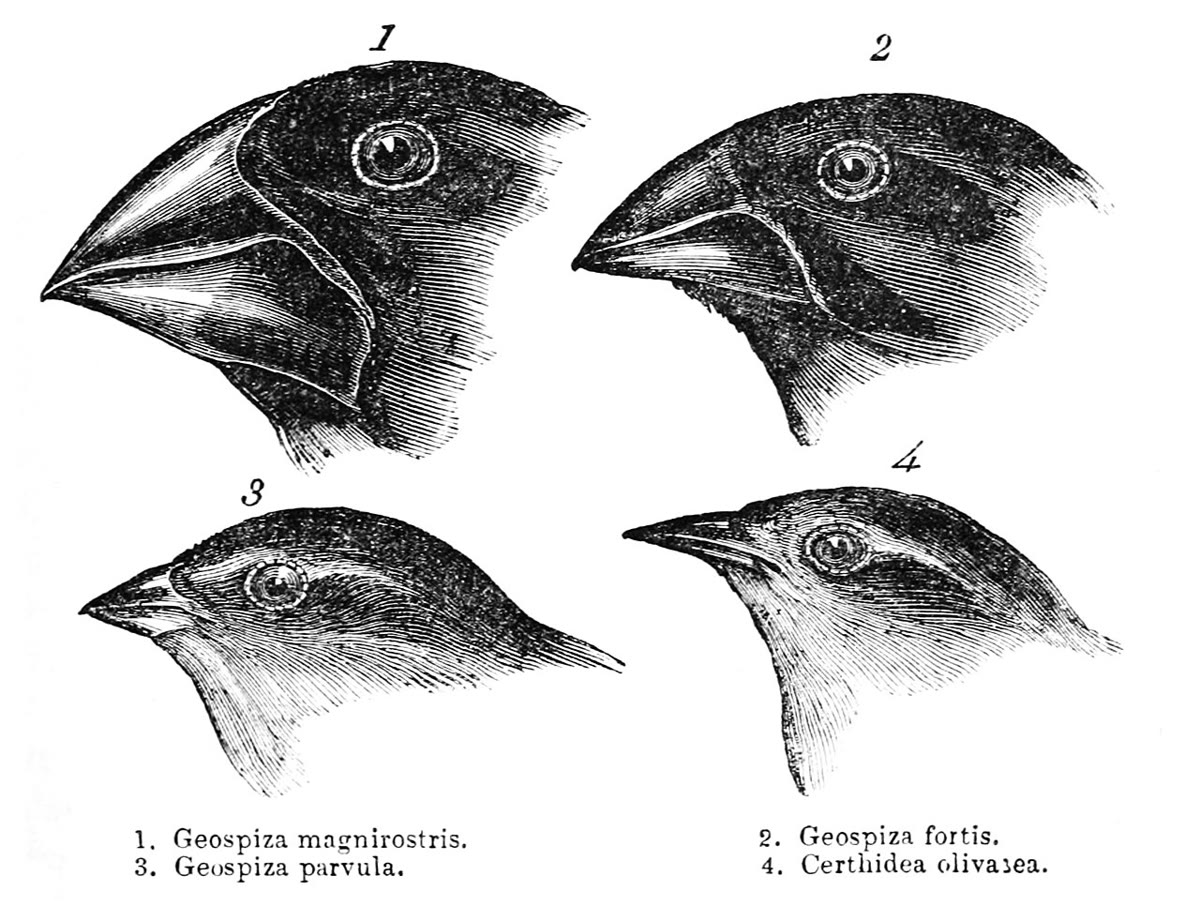
\includegraphics[width=0.62\linewidth]{images/book2/finches-gould.jpg}

{\small أربعة من عصافير داروين، رسمها جون غولد سنة 1845 من العينات التي جلبتها \emph{بيغل}: الطائر نفسه في كل ما عدا ذلك، بمناقير من كسارة الجوز إلى الإبرة. تفصل بينها إشارة نمو واحدة، مجرَّعة على نحو مختلف في الجنين. نقش، ملكية عامة.}
\end{omfigure}

\section{العيش معًا: التعايش}

\begin{definition}[التعايش]\label{def:g12:diversification-of-life:symbiosis}
\emph{التعايش}\index{تعايش} ارتباط دائم وثيق بين نوعين ينتفع به
كلاهما. فالأشنة فطر يؤوي \omterm{def:g10:cells-common-unit:cell}{خلايا} طحلبية تغذيه \omterm{def:g10:cell-metabolism:autotrophy}{بالتركيب الضوئي} بينما
يكنّها ويرويها؛ والمرجان حيوان يؤوي طحالب في أنسجته؛ وجذور معظم
النباتات ملفوفة بفطور تمدها بالأملاح مقابل السكر؛ وأمعاء الحيوانات
تحوي جراثيم تهضم ما لا يستطيع الحيوان هضمه. وينتج الارتباط كائنات
وبنى وأنماط عيش لم يكن أي من الشريكين ليبلغها وحده.
\end{definition}

\begin{omfigure}
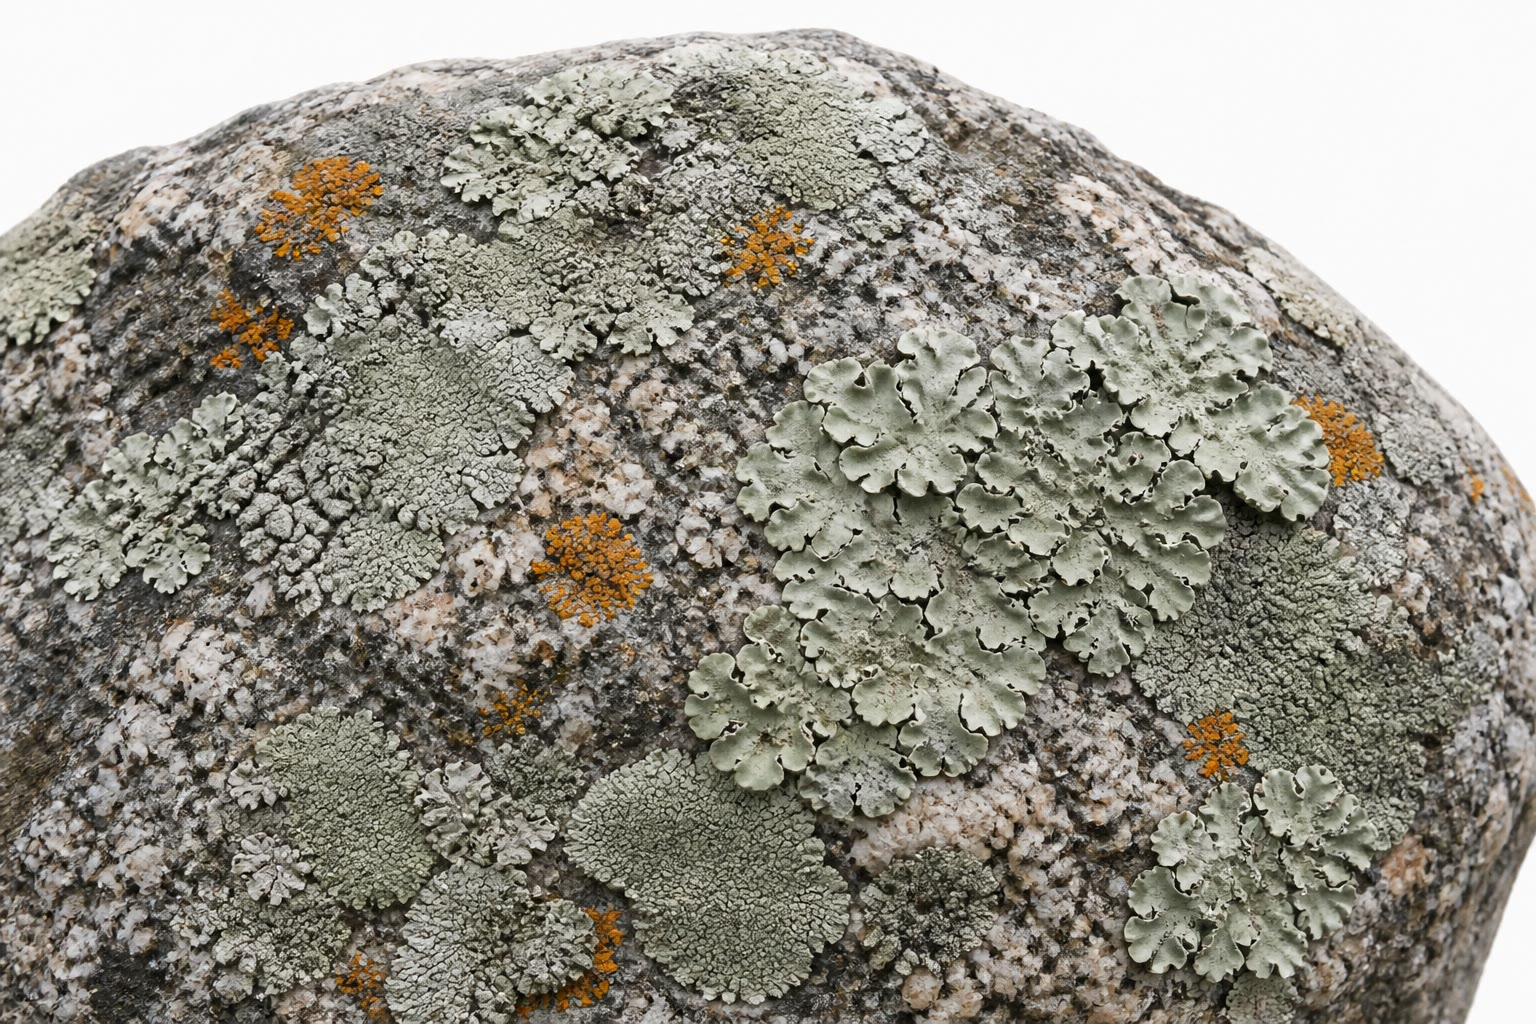
\includegraphics[width=0.58\linewidth]{images/book2/ai/g12-diversif-lichen.jpg}

{\small أشنات على صخرة غرانيتية. كل رقعة فطر وطحلب نبتا جسدًا واحدًا:
صورة من صور الحياة قادرة على استعمار الصخر العاري، لا يقوى عليها أي من
الشريكين وحده.}
\end{omfigure}

\begin{proposition}[التعايش داخل كل خلية]\label{prop:g12:diversification-of-life:endosymbiosis}
متقدرات كل \omterm{def:g10:cells-common-unit:prokaryote}{خلية حقيقية النواة}، وبلاستيدات \omterm{def:g10:cells-common-unit:cell}{الخلايا} النباتية، منحدرة من
جراثيم حرة المعيشة ابتلعتها \omterm{def:g10:cells-common-unit:cell}{خلية} سلفية قبل نحو ملياري سنة فبقيت فيها.
\omterm{def:g10:cells-common-unit:prokaryote}{والخلية حقيقية النواة} نفسها حصيلة \omterm{def:g12:diversification-of-life:symbiosis}{تعايش}.
\end{proposition}
\begin{proof}[شواهد]
للمتقدرات والبلاستيدات \omterm{def:g10:universal-dna:information}{DNA} خاص بها، حلقة صغيرة كحلقة الجرثومة،
وريبوزومات خاصة بها من النمط الجرثومي، حساسة \omterm{def:g11:antibiotic-resistance:antibiotic}{للمضادات الحيوية} التي
تسد \omterm{def:g10:cells-common-unit:organelle}{الريبوزومات} الجرثومية دون ريبوزومات حقيقيات النوا؛ وهي تتكاثر
بالانقسام إلى اثنتين، ولا تستطيع \omterm{def:g10:cells-common-unit:cell}{الخلية} أن تصنعها من جديد؛ وهي ملفوفة
بغشاءين، يشبه داخلهما غشاءً جرثوميًا؛ ومورّثاتها أقرب، في التسلسل، إلى
\omterm{def:g10:universal-dna:gene}{مورّثات} مجموعات بعينها من الجراثيم الحية --- الجراثيم الأرجوانية
للمتقدرات، والجراثيم الزرقاء للبلاستيدات.
\end{proof}

\begin{omfigure}
\begin{tikzpicture}[font=\small, >=Stealth]
  % step 1: large cell + bacterium
  \draw[thick, fill=omDef!8] (0,0) ellipse (1.5 and 1.1);
  \draw[thick, fill=omDef!25] (-0.2,0.1) circle (0.4);
  \draw[thick, fill=omProp!40, rounded corners=4pt] (2.1,-0.15) rectangle (2.9,0.15);
  \node[anchor=north, align=center] at (0,-1.3) {خلية سلفية\\ ذات نواة};
  \node[anchor=north, align=center] at (2.5,-0.4) {جرثومة\\ متنفسة};
  \draw[->, thick] (3.6,0) -- (4.6,0) node[midway, above, font=\scriptsize] {ابتلعت};
  % step 2: bacterium inside
  \begin{scope}[xshift=6.3cm]
    \draw[thick, fill=omDef!8] (0,0) ellipse (1.5 and 1.1);
    \draw[thick, fill=omDef!25] (-0.4,0.15) circle (0.4);
    \draw[thick, fill=omProp!40, rounded corners=4pt] (0.35,-0.5) rectangle (1.15,-0.2);
    \node[anchor=north, align=center] at (0,-1.3) {أبقيت ولم تهضم؛\\ وتنقسم في الداخل};
  \end{scope}
  \draw[->, thick] (8.2,0) -- (9.2,0) node[midway, above, font=\scriptsize, align=center] {ملياران\\ من السنين};
  % step 3: modern cell with mitochondria
  \begin{scope}[xshift=10.9cm]
    \draw[thick, fill=omDef!8] (0,0) ellipse (1.5 and 1.1);
    \draw[thick, fill=omDef!25] (-0.4,0.15) circle (0.4);
    \foreach \x/\y/\r in {0.5/0.4/20, 0.7/-0.3/-40, -0.2/-0.6/70}
      \draw[thick, fill=omProp!40, rotate around={\r:(\x,\y)}] (\x,\y) ellipse (0.3 and 0.13);
    \node[anchor=north, align=center] at (0,-1.3) {خلية حقيقية النواة:\\ متقدرات};
  \end{scope}
\end{tikzpicture}

{\small أصل \omterm{def:g10:cells-common-unit:organelle}{المتقدرات}. جرثومة ابتلعتها \omterm{def:g10:cells-common-unit:cell}{خلية} سلفية فأبقيت وتكاثرت
داخلها؛ ونسلها متقدرات كل حقيقي \omterm{def:g10:cells-common-unit:organelle}{نواة}، وهي ما زالت تحمل \omterm{def:g10:universal-dna:information}{DNA}
وريبوزومات جرثومية خاصة بها. ونشأت البلاستيدات على النحو نفسه من
جرثومة \omterm{def:g10:cell-metabolism:autotrophy}{تركيب ضوئي}.}
\end{omfigure}

\section{تنوّع بلا مورّثات: السلوك}

\begin{proposition}[السلوك المنقول]\label{prop:g12:diversification-of-life:behaviour}
في حيوانات كثيرة، يكون بعض ما يفعله الفرد متعلَّمًا من غيره --- بالتقليد
أو التعليم أو المحاكاة --- ومنقولًا بدوره: أي \emph{ثقافة}\index{ثقافة حيوانية}
تنتقل بلا \omterm{def:g10:universal-dna:gene}{مورّثات}. ومن ثم تستطيع جمهرات \omterm{def:g10:biodiversity-scales:species}{النوع} الواحد أن تختلف
في السلوك كما تختلف في \omterm{def:g10:universal-dna:gene}{الأليلات}، ويستطيع سلوك أن ينتشر في جمهرة في جيل
واحد بدل الأجيال الكثيرة التي تحتاجها \omterm{def:g11:mutations:mutation}{طفرة}.
\end{proposition}
\begin{proof}[شواهد]
جماعات الشمبانزي في غابات مختلفة تستعمل أدوات مختلفة --- حجارة لكسر
الجوز هنا، وعصيًا لاصطياد الأرضة هناك، وأوراقًا كالإسفنج في مكان ثالث
--- والفروق لا تتبع القرابة الوراثية ولا توافر المواد؛ والشمبانزي
الصغير يكتسب طقم جماعته بمشاهدة الكبار. والعصافير المغردة التي تربى
معزولة تغني غناء فجًا؛ فإن ربيت وهي تسمع البالغين غنت لهجة المكان،
وهي تتغير عبر النطاق كما تتغير لهجة البشر. وقطيع من المكاك في جزيرة
تعلم غسل البطاطا الحلوة في البحر من أنثى صغيرة واحدة في غضون عقد، وما
زال نسله يفعل ذلك.
\end{proof}

\begin{omfigure}
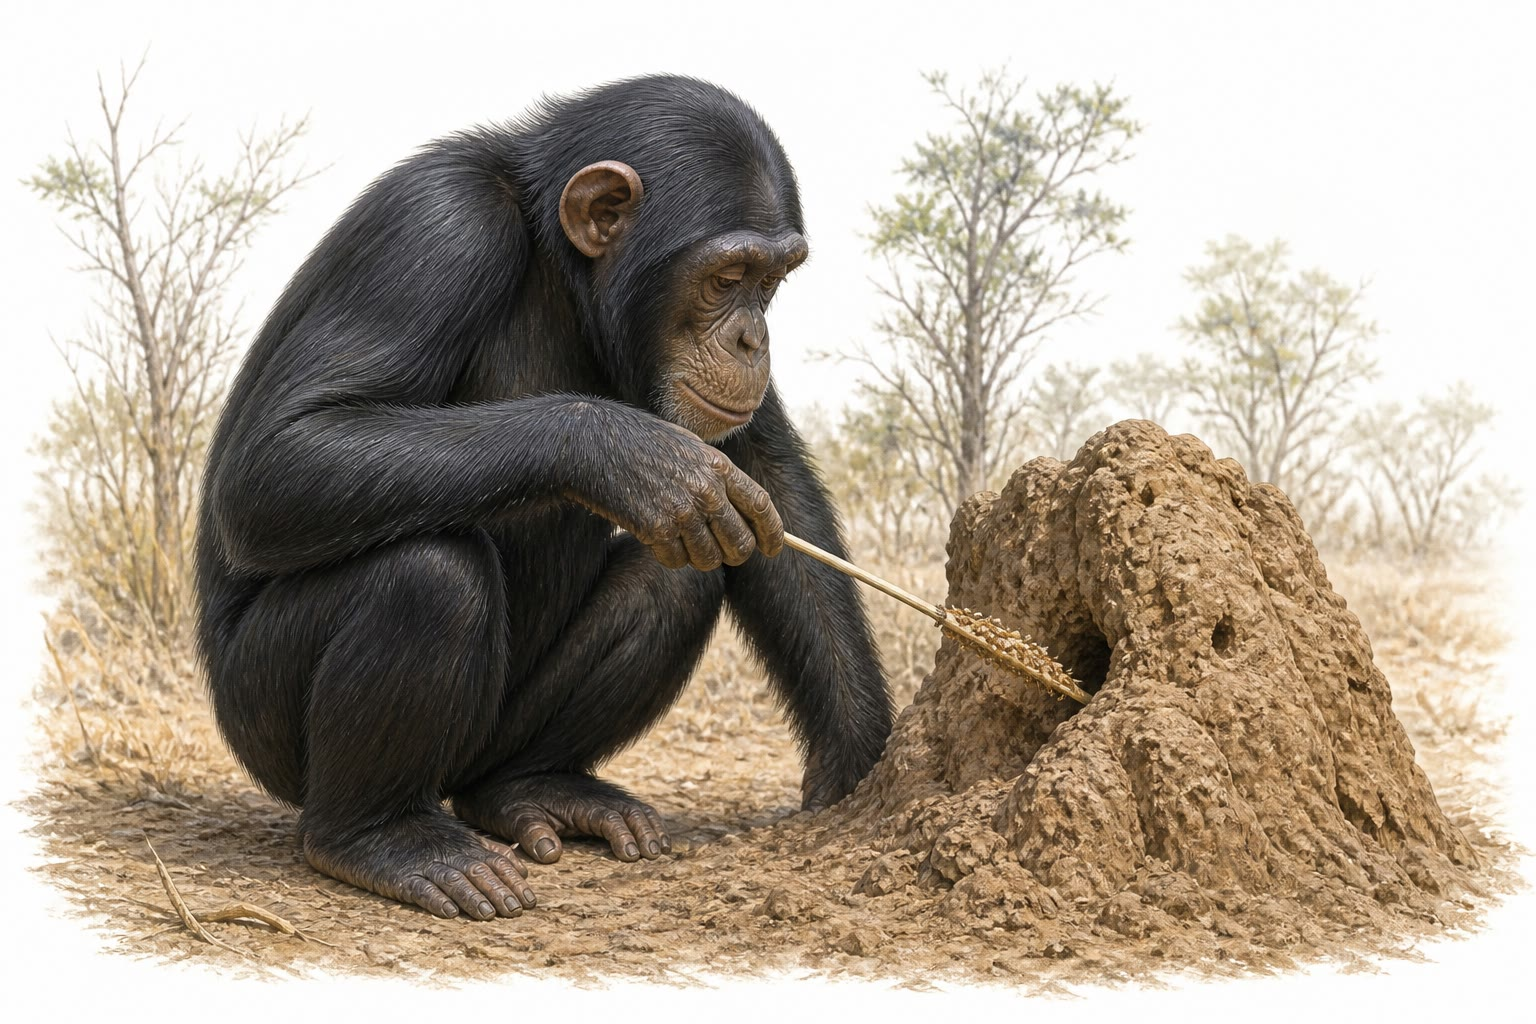
\includegraphics[width=0.6\linewidth]{images/book2/ai/g12-diversif-chimp-tool.jpg}

{\small شمبانزي يصطاد الأرضة بعصًا مهيأة. والتقنية متعلَّمة بالمشاهدة،
وتختلف من جماعة إلى أخرى: تقليد ينتقل بلا \omterm{def:g10:universal-dna:gene}{مورّثات}.}
\end{omfigure}

\begin{method}[تسمية مصدر الفرق]\label{met:g12:diversification-of-life:name}
إذا واجهت فرقًا بين كائنين أو بين جمهرتين:
\begin{enumerate}
  \item أهو في تسلسل \omterm{def:g10:universal-dna:gene}{مورّثة} (\omterm{def:g11:mutations:mutation}{طفرة}، \omterm{def:g10:universal-dna:gene}{أليل})؟ أم في عدد نسخ \omterm{def:g10:universal-dna:gene}{مورّثة}
        (تضاعف)؟ أم في وجود \omterm{def:g10:universal-dna:gene}{مورّثة} من مكان آخر (نقل أفقي)؟ أم في عدد
        الأطقم الصبغية (\omterm{prop:g12:diversification-of-life:polyploidy}{تعدد الصيغ الصبغية})؟
  \item أهو في متى وأين وبأي مقدار يعبَّر عن \omterm{def:g10:universal-dna:gene}{مورّثة} مشتركة أثناء النماء
        (تنظيم)؟
  \item أهو حصيلة ارتباط \omterm{def:g10:biodiversity-scales:species}{بنوع} آخر (\omterm{def:g12:diversification-of-life:symbiosis}{تعايش})؟
  \item أهو متعلَّم (سلوك ينتقل بالثقافة) --- موروث، لكن لا وراثيًا؟
\end{enumerate}
وكثيرًا ما يصح أكثر من جواب؛ والأسئلة هي جرد هذا الفصل.
\end{method}

\begin{remark}[التنوّع والانتقاء]\label{rem:g12:diversification-of-life:selection}
كل مسار هنا ينتج تنوعًا؛ ولا واحد منها يقرر ما ينجو. فقمح \omterm{prop:g12:diversification-of-life:polyploidy}{متعدد الصيغة
الصبغية}، ونمط تعبير عند الأصلة، وأشنة، وتقليد كسر الجوز، بقي كل منها
لأنه نفع حيث نشأ. أما فرز التنوع --- بالانتقاء وبالمصادفة --- فموضوع
الفصل التالي؛ وهذا الفصل قد بسط كم من التنوع يوجد ليفرز، وكم من طريقة
إلى صنعه.
\end{remark}

\section{تمارين}

\begin{exercise}[$\star$]\label{exo:g12:diversification-of-life:1}
اذكر خمسة مصادر للتنوع غير \omterm{def:g11:mutations:mutation}{الطفرة} النقطية.
\end{exercise}

\begin{exercise}[$\star$]\label{exo:g12:diversification-of-life:2}
ما \omterm{prop:g12:diversification-of-life:duplication}{العائلة المورّثية}، وكيف تنشأ؟
\end{exercise}

\begin{exercise}[$\star$]\label{exo:g12:diversification-of-life:3}
لماذا يكون الهجين بين نوعين عقيمًا عادة، وكيف تستطيع مضاعفة \omterm{def:g10:universal-dna:information}{الصبغيات}
أن تجعله خصيبًا؟
\end{exercise}

\begin{exercise}[$\star$]\label{exo:g12:diversification-of-life:4}
أعط ثلاثة شواهد على أن \omterm{def:g10:cells-common-unit:organelle}{المتقدرات} منحدرة من جراثيم.
\end{exercise}

\begin{exercise}[$\star$]\label{exo:g12:diversification-of-life:5}
ما المقصود بالثقافة عند الحيوان؟ أعط مثالًا.
\end{exercise}

\begin{exercise}[$\star\star$]\label{exo:g12:diversification-of-life:6}
للقمح ثنائي الحبة $2n = 28$ وللأحادية $2n = 14$. كم صبغيًا لهجينهما،
وكم زوجًا يستطيع أن يتكون في انقسامه المنصّف؟ فسّر عقمه.
\end{exercise}

\begin{exercise}[$\star\star$]\label{exo:g12:diversification-of-life:7}
مورّثتا الغلوبين $\alpha$ و$\beta$ متطابقتان بنسبة 50\%؛ والمورّثتان
$\beta$ و$\gamma$ بنسبة 80\%. أي التضاعفين أقدم؟ ارسم الشجرة.
\end{exercise}

\begin{exercise}[$\star\star$]\label{exo:g12:diversification-of-life:8}
فسّر كيف تكون الأصلة بلا أرجل مع أنها تحمل \omterm{def:g10:universal-dna:gene}{المورّثات} التي تبني الأرجل
عند السحلية.
\end{exercise}

\begin{exercise}[$\star\star$]\label{exo:g12:diversification-of-life:9}
نوعان من العصافير يختلف عمق منقاريهما بمعامل قدره اثنان، \omterm{def:g10:universal-dna:gene}{ومورّثات}
منقاريهما متطابقة. أين يقع الفرق، ولماذا أمكن أن ينشأ سريعًا؟
\end{exercise}

\begin{exercise}[$\star\star$]\label{exo:g12:diversification-of-life:10}
أشنة تنبت من فطرها وحده عفن بلا شكل؛ ومن طحلبها وحده غشاء أخضر. فسّر
بأي معنى تكون الأشنة صنفًا جديدًا من الكائنات.
\end{exercise}

\begin{exercise}[$\star\star$]\label{exo:g12:diversification-of-life:11}
جمهرة من الشمبانزي تكسر الجوز؛ وجمهرة مجاورة، عبر نهر، لا تكسره، مع
أن الجوز والحجارة وافران على الضفتين. مستعينًا بالطريقة في
\cref{met:g12:diversification-of-life:name}، عيّن مصدر الفرق وبرهن.
\end{exercise}

\begin{exercise}[$\star\star\star$]\label{exo:g12:diversification-of-life:12}
\omterm{def:g10:universal-dna:gene}{مورّثة} من المجين البشري تكاد تطابق \omterm{def:g10:universal-dna:gene}{مورّثة} فيروس ولا تشبه شيئًا في أي
ثديي آخر عدا الرئيسيات. اقترح تاريخها، وقل كيف تختبره.
\end{exercise}

\begin{exercise}[$\star\star\star$]\label{exo:g12:diversification-of-life:13}
\omterm{def:g11:antibiotic-resistance:antibiotic}{المضادات الحيوية} التي تسد \omterm{def:g10:cells-common-unit:organelle}{الريبوزومات} الجرثومية لها آثار جانبية في
متقدرات المريض عند الجرعات العالية. فسّر لماذا، وماذا يقول ذلك عن أصل
\omterm{def:g10:cells-common-unit:organelle}{المتقدرات}.
\end{exercise}

\begin{exercise}[$\star\star\star$]\label{exo:g12:diversification-of-life:14}
فسّر لماذا يكون \omterm{def:g10:biodiversity-scales:species}{نوع} \omterm{prop:g12:diversification-of-life:polyploidy}{متعدد الصيغة الصبغية} جديد معزولًا عن أبويه من الجيل
الأول، بينما يحتاج \omterm{def:g10:universal-dna:gene}{أليل} جديد أجيالًا كثيرة لينتشر. وماذا يستلزم ذلك في
سرعة تكوّن \omterm{def:g10:biodiversity-scales:species}{الأنواع} النباتية؟
\end{exercise}

\begin{exercise}[$\star\star\star$]\label{exo:g12:diversification-of-life:15}
"كل تنوّع آت من \omterm{def:g11:mutations:mutation}{الطفرة}." ناقش في فقرة: بأي معنى تصح العبارة في الأساس،
وبأي معان تتجاوزها مسارات هذا الفصل.
\end{exercise}

\section{مسألة: ثلاث حشائش في رغيف}

\begin{problem}[{مسألة نهاية الأسبوع --- تاريخ قمح الخبز يعاد بناؤه من
الصبغيات، ومورّثات الأصلة تقرأ إلى جانب مورّثات الفأر، والجرثومة التي
في كل خلية تحاكم}]
\label{pb:g12:diversification-of-life:1}
للأحادية (AA) ولعشبة الماعز 1 (BB) ولعشبة الماعز 2 (DD) لكل منها
$2n = 14$. والقمح ثنائي الحبة AABB وقمح الخبز AABBDD.

\medskip
\noindent\textbf{القسم الأول --- صبغيات القمح.}
\begin{enumerate}
  \item أعط عدد \omterm{def:g10:universal-dna:information}{الصبغيات} في القمح ثنائي الحبة وفي قمح الخبز.
  \item لهجين الأحادية وعشبة الماعز 1 أربعة عشر صبغيًا، سبعة من كل
        صنف. كم زوجًا من المتماثلات يتكون في انقسامه المنصّف؟ وكيف
        تكون أمشاجه؟
  \item فسّر لماذا تعيد مضاعفة صبغياته الخصوبة: أحص الأزواج.
  \item لهجين القمح ثنائي الحبة وعشبة الماعز 2 واحد وعشرون صبغيًا.
        أيها يستطيع أن يتزاوج، ولماذا كان عقيمًا؟
  \item بعد المضاعفة، لقمح الخبز 42. كم زوجًا يتكون في انقسامه
        المنصّف، وكم صبغيًا تحمل حبة الطلع؟
\end{enumerate}

\medskip
\noindent\textbf{القسم الثاني --- قراءة التاريخ.}
\begin{enumerate}[resume]
  \item يحمل قمح الخبز ثلاث نسخ من معظم \omterm{def:g10:universal-dna:gene}{المورّثات}، واحدة على كل طقم.
        فسّر لماذا لا يكون \omterm{def:g11:mutations:mutation}{لطفرة} تتلف نسخة واحدة أثر مرئي عادة، وماذا
        يتيح ذلك مع الزمن.
  \item زرع القمح ثنائي الحبة قبل 10\,000 سنة، ويظهر قمح الخبز في
        المواقع الأثرية قبل 8\,000 سنة. فأين ومتى وقع التهجين الثاني
        على الأرجح؟ وما الذي كان لا بد أن ينبت جنبًا إلى جنب؟
  \item تهجينات مختبرية للقمح ثنائي الحبة مع عشبة الماعز 2، تتبعها
        مضاعفة كيميائية، تعطي نباتات خصيبة تشبه قمح الخبز. أي نتيجة من
        نتائج هذا التاريخ يؤكد ذلك؟
  \item لا يستطيع قمح الخبز أن يتهاجن مع الأحادية فيعطي نسلًا خصيبًا.
        أهو \omterm{def:g10:biodiversity-scales:species}{نوع} مستقل؟ برهن بتعريف \cref{ch:g10:biodiversity-scales}.
  \item مربّي محاصيل يريد إدخال \omterm{def:g10:universal-dna:gene}{مورّثة} مقاومة لمرض من عشبة الماعز 2
        إلى قمح الخبز. فسّر لماذا كان هذا أيسر من إدخالها من نبات غير
        قريب.
\end{enumerate}

\medskip
\noindent\textbf{القسم الثالث --- \omterm{def:g10:universal-dna:gene}{مورّثات} الأصلة.}
\begin{enumerate}[resume]
  \item \omterm{def:g10:universal-dna:gene}{المورّثات} المجالية للجذع متطابقة بنسبة 98\% بين الفأر والأصلة.
        ماذا يقول ذلك عن مصدر الفرق بين جسديهما؟
  \item في جنين الفأر تنشط \omterm{def:g10:universal-dna:gene}{مورّثة} "الجذع المضلع" على 13 قطعة؛ وفي
        الأصلة على نحو 300. سمّ نمط التغير المعني.
  \item يكوّن جنين الأصلة براعم ضئيلة حيث كانت الأطراف الخلفية تكون،
        ثم تكف عن النمو. ماذا يوحي ذلك عن \omterm{def:g10:universal-dna:gene}{مورّثات} الأطراف وعن الإشارة
        التي كانت ستنشطها؟
  \item الفئران المهندسة للتعبير عن \omterm{def:g10:universal-dna:gene}{مورّثة} "الجذع المضلع" على المجال
        القطني تنبت هناك أضلاعًا زائدة. ماذا تضيف هذه التجربة إلى
        المقارنة؟
  \item قارن نمطي التغير: تغير قمح الخبز وتغير الأصلة. أيهما غيّر حجم
        المجين، وأيهما غيّر استعماله؟
\end{enumerate}

\medskip
\noindent\textbf{القسم الرابع --- الجرثومة التي في الداخل.}
\begin{enumerate}[resume]
  \item اذكر أربع سمات للمتقدرات توافق أصلًا جرثوميًا، وقل عند كل واحدة
        ماذا كنت تتوقع لو كانت \omterm{def:g10:cells-common-unit:cell}{الخلية} قد بنت \omterm{def:g10:cells-common-unit:organelle}{المتقدرات} من الصفر.
  \item لا يحمل \omterm{def:g10:universal-dna:information}{DNA} \omterm{def:g10:cells-common-unit:organelle}{المتقدرة} إلا 37 \omterm{def:g10:universal-dna:gene}{مورّثة}، مع أن \omterm{def:g10:cells-common-unit:organelle}{المتقدرة} تحتاج نحو
        1500 \omterm{def:g11:gene-expression:protein}{بروتين}. فأين \omterm{def:g10:universal-dna:gene}{المورّثات} الأخرى، وماذا جرى لها على مدى
        ملياري سنة؟
  \item كل \omterm{def:g10:cells-common-unit:organelle}{متقدرة} عند الإنسان آتية من البييضة، ولا واحدة من المنوي.
        فماذا يترتب على ذلك في توارث \omterm{def:g10:universal-dna:gene}{مورّثات} \omterm{def:g10:cells-common-unit:organelle}{المتقدرة}، وفي تتبع النسب
        الأمومي؟
  \item الأشنة \omterm{def:g10:cells-common-unit:organelle}{والمتقدرة} كلتاهما \omterm{def:g12:diversification-of-life:symbiosis}{تعايش}. فبأي وجه ذهب \omterm{def:g12:diversification-of-life:symbiosis}{تعايش} \omterm{def:g10:cells-common-unit:organelle}{المتقدرة}
        أبعد؟
  \item اذكر النتيجة: \omterm{def:g10:biodiversity-scales:species}{الأنواع} الثلاثة التي في الرغيف وعدد \omterm{def:g10:universal-dna:information}{الصبغيات}
        التي أسهم بها كل منها؛ والكلمة الواحدة التي تسمي ما يختلف بين
        استعمال الأصلة واستعمال الفأر لمورّثاتهما المشتركة؛
        \omterm{def:g10:cells-common-unit:organelle}{والعضية} التي كانت جرثومة.
\end{enumerate}
\end{problem}
